\subsection{Theory}
%%%%%%%%%%%%%%%%%%%%%%%%%%%%%%%%%%%%%%%%%%%%%%%%%%%%%%%%%%%%%%%%%%%%%
% \begin{frame}{Capabilities of a single agent (Robot)}
% \begin{itemize}
% 	\item Position information based on an indoor positioning system (can be relaxed to only distance measurements)
% 	\item Peer to peer communication and computation capabilites onboard
% 	\item Pretend to measure the strength of a virtual scalar field based on the current location
% \end{itemize}		
% \end{frame}
%%%%%%%%%%%%%%%%%%%%%%%%%%%%%%%%%%%%%%%%%%%%%%%%%%%%%%%%%%%%%%%%%%%%%
\begin{frame}{Source seeking problem as optimization}
\begin{itemize} 
	\item Look at the source seeking problem as a minimization problem
	\item Momentum methods\footnote{Polyak,1964} have been used in optimization to speed up or dampen the oscillations
	\item Naturally have momentum of the mobile robots   
	\item For theoretical analysis: Use continuous-time versions of optimization methods to study the assymptotic properties\footnote{Redont et al., 2002} 
\end{itemize}
\end{frame}
% %%%%%%%%%%%%%%%%%%%%%%%%%%%%%%%%%%%%%%%%%%%%%%%%%%%%%%%%%%%%%%%%%%%%%
% \begin{frame}{Continuous-time steepest descent with momentum}
% \begin{itemize}
% \item Consider the problem of minimizing a differentiable $f:\mathbb{R}^n\rightarrow \mathbb{R}$
% \pause
% \item The steepest descent iteration is
% \begin{equation}
% x_{k+1}=x_k - \alpha \nabla f(x_k)
% \end{equation}
% \pause
% \item The continuous-time version of the steepest descent dynamics 
% \begin{equation}
% \dot{x}= - \nabla f(x_k)
% \end{equation}
% \pause
% \item The continuous-time version of the steepest descent dynamics with momentum (also known as the heavy ball method with friction) 
% \begin{equation}
% m\ddot{x}+ \dot{x}= - \nabla f(x_k)
% \end{equation}
% \end{itemize}
% \end{frame}
%%%%%%%%%%%%%%%%%%%%%%%%%%%%%%%%%%%%%%%%%%%%%%%%%%%%%%%%%%%%%%%%%%%%%
\begin{frame}{Continuous-time Newton method with momentum}
\begin{itemize}
	\item Consider the problem of minimizing a twice-differentiable, strongly convex $f:\mathbb{R}^n\rightarrow \mathbb{R}$
	\pause
	\item The Newton iteration is
	\begin{equation}
	x_{k+1}=x_k - \alpha\nabla^2f(x_k)^{-1} \nabla f(x_k)
	\end{equation}
	\pause
	\item The continuous-time version of these dynamics can be represented as
	\begin{equation}
	\nabla^2f(x_k)\dot{x}= - \nabla f(x_k)
	\end{equation}
	\pause
	\item Adding momentum to these dynamics gives  
	\begin{equation}
	m\ddot{x}+ \nabla^2f(x_k)\dot{x}= - \nabla f(x_k)
	\end{equation}
\end{itemize}
\pause
Defining the velocity variable $v$, the dyanmics can be written as 
\begin{equation} \label{eqn: second_order_newton_cont_time}
\begin{split}
\Dot{x}&=v\\
\Dot{v}&=-k_1\nabla^2 f(x) v -k_2 \nabla f(x), 
\end{split}
\end{equation}
\end{frame}
%%%%%%%%%%%%%%%%%%%%%%%%%%%%%%%%%%%%%%%%%%%%%%%%%%%%%%%%%%%%%%%%%%%%%
\begin{frame}{Flocking and schooling in nature}

\begin{minipage}{0.45\textwidth}	
	%\hspace{0.4cm}	
	\begin{figure}
		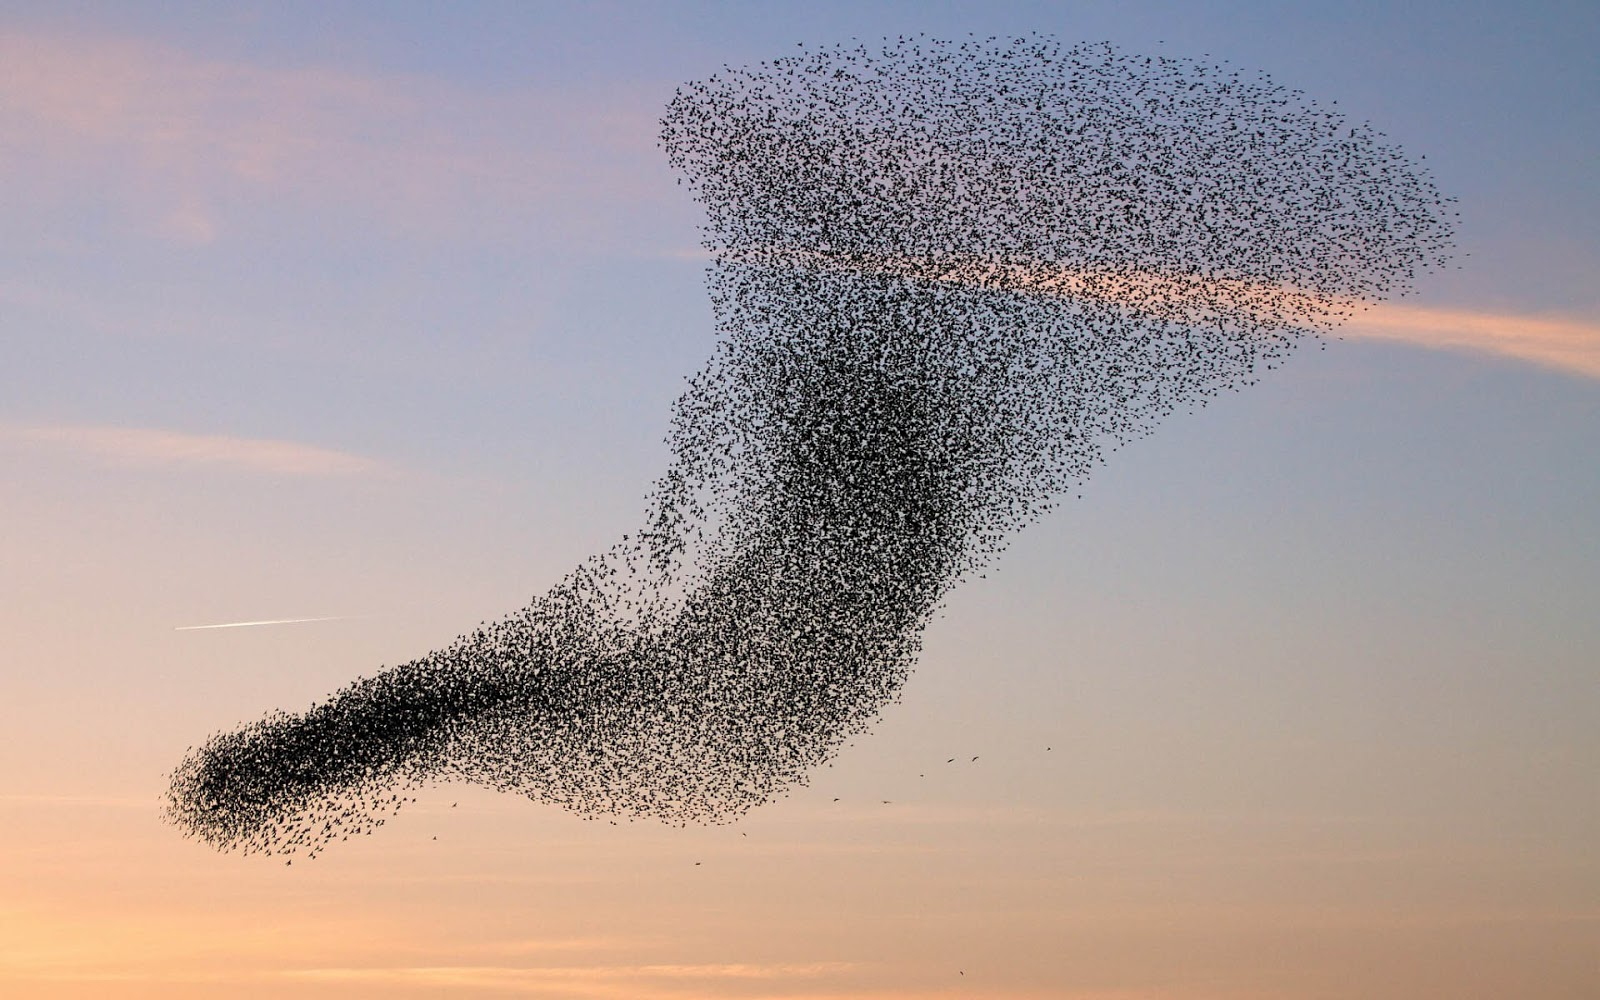
\includegraphics[width=\textwidth]{figures/flock_of_birds.jpg}
		%\caption{Fukushima Disaster}
		%\label{fig:flock_of_birds}
	\end{figure}
\end{minipage}
\hspace{0.05cm}
\begin{minipage}{0.45\textwidth}	
	\begin{figure}
		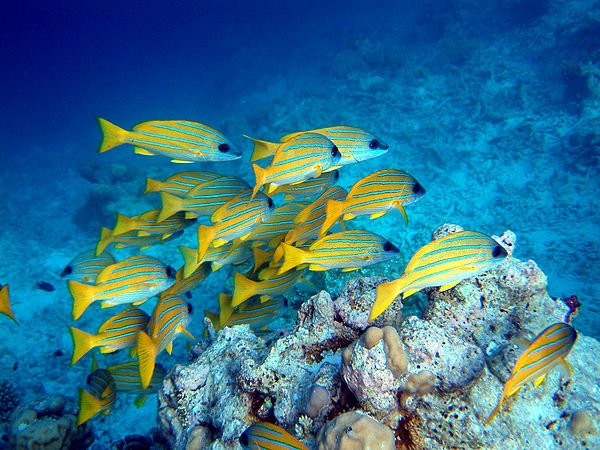
\includegraphics[width=\textwidth]{figures/schooling_fish.jpg}
		%\caption{Oil Spills}
		%\label{fig:schools_of_fish}
	\end{figure}
\end{minipage}
\begin{itemize}	
	\item The precise rules that these animals use are not known
	\item Particle-based flocking seems to be an effective approach to model such behavior
	\item In 1987, Reynold was working on animating flocking behavior where he proposed three rule
	\begin{itemize}
		\item Cohesion: Attempt to stay close to nearby neighbors
		\item Separation: Avoid collisions with nearby flockmates
		\item Alignment: attempt to match velocities with nearby flockmates
	\end{itemize}
\end{itemize}
\end{frame}
%%%%%%%%%%%%%%%%%%%%%%%%%%%%%%%%%%%%%%%%%%%%%%%%%%%%%%%%%%%%%%%%%%%%%
\begin{frame}{Flocking dynamics}
\begin{itemize}
	\item Every particle interacts with every other particle based on an interaction field $V$ which depends only on the distance between them
	\item An example of a potential field is the gravitational field $V(z)=\frac{mMG}{||z||}$
	\item Flocking dynamics\footnote{Olfati-Saber, 2004}:
	\begin{equation*}
	\begin{split}
	\Dot{q}&=p\\
	\Dot{p}&=-\nabla V(q)-\hat{L}(q)p -cp 
	\end{split}
	\end{equation*}
\end{itemize}
\end{frame}
%%%%%%%%%%%%%%%%%%%%%%%%%%%%%%%%%%%%%%%%%%%%%%%%%%%%%%%%%%%%%%%%%%%%%
\begin{frame}{Flocking towards the source}
\begin{itemize}
\item Consider now an underlying source field $\psi:\mathbf{R}^m \xrightarrow{} \mathbf{R}$ which is smooth enough and convex.
\item Add a forcing term to the flocking dynamics motivated from the discussion on optimization
\item Flocking dynamics with source-seeking:
\begin{equation*}
\begin{split}
\Dot{q}&=p\\
\Dot{p}&=-\nabla V(q)-\hat{L}(q)p -cp\textcolor{red}{-k_1\nabla^2 \Psi(q) p -k_2 \nabla \Psi(q)}
\end{split}
\end{equation*}
\end{itemize}
\end{frame}
%%%%%%%%%%%%%%%%%%%%%%%%%%%%%%%%%%%%%%%%%%%%%%%%%%%%%%%%%%%%%%%%%%%%%
\begin{frame}{Stability(Convergence) Analysis}
	Flocking dynamics with source-seeking:
	\begin{equation*}
	\begin{split}
	\Dot{q}&=p\\
	\Dot{p}&=-\nabla V(q)-\hat{L}(q)p -cp\textcolor{red}{-k_1\nabla^2 \Psi(q) p -k_2 \nabla \Psi(q)}
	\end{split}
	\end{equation*}
\textbf{Theorem 1} For twice differentiable convex fields $\psi:\mathbf{R}^m \xrightarrow{} \mathbf{R}$, the above flocking dynamics are stable i.e the trajectories remain bounded. Moreover, for all initial conditions $(q(0),p(0))$, the trajectories converge asymptotically to the set $$\mathcal{W}:=\{(q^*,0)|\nabla V (q^*)+ k_2\nabla\Psi(q^*) = 0 \}.$$
%% Additionally, if $\psi$ is radially symmetric about the source $q_s$, then, at the equilibrium of the translational dynamics of the center of mass, (?), $q_s \in \textnormal{convhull}(q^*)$  
\textbf{Corollary 1} Assume, the field $\psi:\mathbf{R}^m \xrightarrow{} \mathbf{R}$ is strictly convex, quadratic and has a unique minimum located at $q_s$, we have that $\lim_{t\rightarrow \infty}q_c(t)=q_s$.

\end{frame}
%%%%%%%%%%%%%%%%%%%%%%%%%%%%%%%%%%%%%%%%%%%%%%%%%%%%%%%%%%%%%%%%%%%%%%
%\begin{frame}{Stability(Convergence) Analysis}
%\textbf{Proof:}
%	\begin{itemize}
%		\item Define the energy function
%		\begin{equation*}\label{eqn: energy function}
%		E(t):= V(q(t)) + k_2\Psi(q(t)) + \frac{1}{2}p(t)^Tp(t).
%		\end{equation*}
%		%\pause
%		\item Differentiating w.r.t time, 
%		\begin{equation*}
%		\begin{split}
%		\dot{E}&= (\nabla V(q) + k_2\nabla \Psi(q))^T\dot{q} + p^T\dot{p} \\
%		&=-p^T(\hat{L}(q)+cI+k_1\nabla^2\Psi(q))p\\
%		&\leq 0.
%		\end{split}
%		\end{equation*}
%		%\pause
%		\item $E(t)\leq E(0) ~\forall t\geq0$ implies the boundedness of trajectories
%		%\pause
%		\item  $\dot{E}=0 \iff p=0$. Thus, LaSalle's invariance principle $\implies$ that the trajectories converge to the largest invariant set contained in $\mathcal{W}:=\{(q^*,0)|\nabla V (q^*)+ k_2\nabla \Psi(q^*) = 0 \}$
%		%\pause
%		%\item At equilibrium of the center of mass dynamics, $q^*$ satisfies $\frac{k_2}{N}(\mathbf{1}_N\otimes I_m)^T\nabla\Psi(q)$
%	\end{itemize}
%\end{frame}
%%%%%%%%%%%%%%%%%%%%%%%%%%%%%%%%%%%%%%%%%%%%%%%%%%%%%%%%%%%%%%%%%%%%%
% \begin{frame}{Stability(Convergence) Analysis}
% 	\textbf{Sketch of the proof(ctd):}
% 	\begin{itemize}
% 		\item To characterize the equilibrium, we write the dynamics of the center of mass
% 		\begin{equation} \label{eqn: COM flocking dynamics}
% 		\begin{split}
% 		\Dot{q}_c&=p_c\\
% 		\Dot{p}_c&=-cp_c-\frac{1}{N}(\mathbf{1}_N\otimes I_m)^T(k_1\nabla^2\Psi(q) p +k_2 \nabla\Psi(q)) 
% 		\end{split}
% 		\end{equation}
% 		\pause
% 		\item $\lim_{t\rightarrow \infty}p(t)=0 \implies \lim_{t\rightarrow \infty}p_c(t)=0$
		
% 	\end{itemize}
% \end{frame}
%%%%%%%%%%%%%%%%%%%%%%%%%%%%%%%%%%%%%%%%%%%%%%%%%%%%%%%%%%%%%%%%%%%%%
%\begin{frame}{Stability(Convergence) Analysis}
%\textbf{Corollary 1} Assume, the field $\psi:\mathbf{R}^m \xrightarrow{} \mathbf{R}$ is strictly convex, quadratic and has a unique minimum located at $q_s$, we have that $\lim_{t\rightarrow \infty}q_c(t)=q_s$.
%
%%\pause
%\textbf{Proof:}
%	\begin{itemize}
%	    \item For quadratic $\psi(q)=\frac{1}{2}q^THq+g^Tq+c_0$, with $H\succ 0$, the source is the unique solution to $Hq_s+g=0$
%		%\pause
%	    \item The center of mass dynamics are governed by
%		    \begin{equation} \label{eqn: COM flocking dynamics}
%        		\begin{split}
%        		\Dot{q}_c&=p_c\\
%        		\Dot{p}_c&=-cp_c-\frac{1}{N}(\mathbf{1}_N\otimes I_m)^T(k_1\nabla^2\Psi(q) p +k_2 \nabla\Psi(q)) 
%        		\end{split}
%		    \end{equation}
%	    %\pause
%	    \item $\frac{1}{N}(\mathbf{1}_N\otimes I_m)^T\nabla\Psi(q)=0$
%		%\pause
%		\item At equilibrium $q^*$, 
%		\begin{equation*}
%		\begin{split}
%		\frac{1}{N}\sum_{i=1}^{N}\nabla\psi(q_i^*)&=0 \iff \textnormal{i.e } H(\frac{1}{N}\sum_{i=1}^{N}q_i^*)+g=0\\
%		\textnormal{i. e  } Hq_c^*+g&=0 \iff q_c^*=q_s
%		\end{split}	
%		\end{equation*}
%		\end{itemize}
%\end{frame}